\section{La bouteille de Klein $K$}
\subsection{Définitions}
La bouteille de Klein, objet classique mais déroutant, se définit en recollant $2$ bandes de Möbius le long de leur bord respectif. On définit la bande de Möbius comme étant $I^2/\mathcal{R}$ avec $\mathcal{R}$ la relation d'équivalence engendrée par $(t,0)\sim(1-t,1),t\in I$. On va ici travailler sur une définition différente de la bouteille de Klein, qui engendre le même objet (à homéomorphisme près). Il s'agira de $I^2/R$ avec $R$ la relation d'équivalence engendrée par $(t,0)\sim(t,1),t\in I$ et $(0,t)\sim(1,1-t),t\in I$. Le schéma ci-dessous explicite l'équivalence de l'un et l'autre :
\begin{figure}[ht]
    \centering
    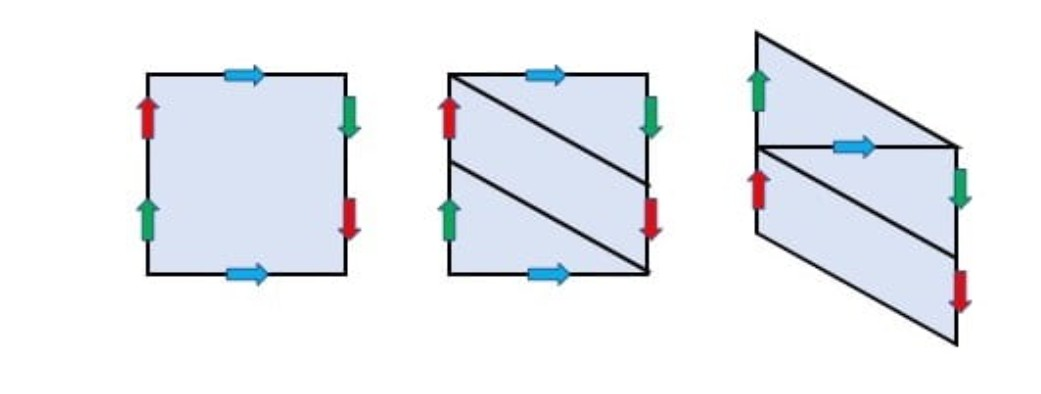
\includegraphics[width=0.5\textwidth]{images/Klein carré.jpg}
\end{figure}
\bigskip\\
\subsection{Calcul de $\pi_1(K)$}
On peut déduire des résultats intéressants à partir de la présentation de $\pi_1(K)$, qu'on va donc d'abord traiter.
\begin{proposition}
    $\pi_1(K)$ est isomorphe à $\langle a,b\mid aba^{-1}b=1\rangle$
\end{proposition}
\begin{proof}
    On répète encore et encore le même procédé à partir de tous les résultats précédents (y compris la Prop. 2.4., car les coins de $K$ s'identifient tous entre eux) : $\pi_1(K)\cong\tilde{V}_0/N\cong\mathbb{Z}*\mathbb{Z}/\phi(N)$\medskip\\
    Notant $\alpha=[t\to[(t,0)]]$ et $\beta=[t\to[(1,t)]]$, on obtient que $i_{\tilde{V}_0}(c_0)=\alpha\beta\alpha^{-1}\beta$ et pour $\phi:\pi_1(\tilde{V}_0)\to\mathbb{Z}*\mathbb{Z}$ l'isomorphisme usuel, on trouve $\phi(i_{\tilde{V}_0}(c_0))=aba^{-1}b$ d'où $\phi(N)=\langle\langle aba^{-1}b\rangle\rangle$.\medskip\\
    Dès lors, par le \textbf{Corollaire 2.2.}, on obtient $\pi_1(K)\cong\mathbb{Z}*\mathbb{Z}/\phi(N)=\mathbb{Z}*\mathbb{Z}/\langle\langle aba^{-1}b\rangle\rangle\cong\langle a,b\mid aba^{-1}b=1\rangle$.
\end{proof}
Ce groupe n'est pas directement identifiable à un produit de copies de $\mathbb{Z}$ ou à un quotient classique comme avec les cas de $T^2$ et $\mathbb{R}$P$^2$. Cependant, on peut en tirer différentes propriétés, qu'on étudie ci-dessous.
\begin{proposition}
    Le produit semi-direct $\mathbb{Z}\times_{\varphi}\mathbb{Z}$ admet la présentation $\langle a,b\mid aba^{-1}b=1\rangle$ avec\\ $\varphi:\mathbb{Z}\to\text{Aut}(\mathbb{Z})$ tel que $(\varphi(n))(m)=(-1)^nm$
\end{proposition}
\begin{proof}
    Il suffit de montrer  :\\
    $i)$ $a=(0,1)$ et $b=(1,0)$ génèrent $\mathbb{Z}\times_{\varphi}\mathbb{Z}$\\ $ii)$ $aba^{-1}b=(0,0)$ l'élément neutre de $\mathbb{Z}\times_{\varphi}\mathbb{Z}$.\medskip\\$i)$ : Montrons que tout élément de $\mathbb{Z}\times\mathbb{Z}$ s'écrit sous la forme $(i,j)=b^ia^j$. Premièrement, $(x,0)*_{\varphi}(y,0)=(x+\varphi(0)(y),0+0)=(x+y,0)$ et par $b^{-1}=(-1,0)$ et une récurrence immédiate, $(i,0)=b^i,i\in\mathbb{Z}$. D'autre part, $(0,x)*_{\varphi}(0,y)=(0+\varphi(x)(0),x+y)=(0,x+y)$ et $a^{-1}=(0,-1)$, d'où $(0,j)=a^j,j\in\mathbb{Z}$.\\
    Ainsi, $b^ia^j=(i,0)*_{\varphi}(0,j)=(i+\varphi(0)(0),0+j)=(i,j)$, d'où le résultat.\medskip\\
    $ii)$ : On a $ab=(0,1)*_{\varphi}(1,0)=(0+\varphi(1)(1),1+0)=(-1,1)$, et $aba^{-1}=(-1,1)*_{\varphi}(0,-1)=(-1,0)$, et enfin $aba^{-1}b=(-1,0)*_{\varphi}(1,0)=(0,0)$, ce qui conclut.
\end{proof}
\begin{proposition}
    $\pi_1(K)$ n'est pas abélien, et son abélianisé est isomorphe à $\mathbb{Z}\times\mathbb{Z}/2\mathbb{Z}$
\end{proposition}
\begin{proof}
    On a $\pi_1(K)\cong\langle a,b\mid aba^{-1}b=1\rangle$, et ce groupe n'est pas abélien car $ab=b^{-1}a\neq ba$ car $b^2\neq 1$. De plus, $\langle a,b\mid aba^{-1}b=aba^{-1}b^{-1}=1\rangle$, l'abélianisé, vérifie alors $b^2=1$ car $b^{-1}a=ba$ et tout élément se réduit à la forme $a^ib^j,i\in\mathbb{Z},j\in\{0,1\}$, offrant un isomorphisme évident à $\mathbb{Z}\times\mathbb{Z}/2\mathbb{Z}$ ($a$ restant libre après abélianisation).  
\end{proof}
